% main.tex — master file for the spinal-fairness paper (LLNCS / Springer LNCS)
% Build: latexmk -pdf main.tex   (runs pdflatex -> bibtex -> pdflatex x2)
% Structure:
%   sections/  — one .tex per section, pulled in via \input below
%   figures/   — media (declared on \graphicspath so \includegraphics needs no prefix)
%   template/  — Springer boilerplate docs (not used in the build)
%
\documentclass[runningheads,a4paper]{llncs}
%
\usepackage[T1]{fontenc}
% T1 fonts will be used to generate the final print and online PDFs,
% so please use T1 fonts in your manuscript whenever possible.
% Other font encondings may result in incorrect characters.
%
\usepackage{graphicx}
% Used for displaying a sample figure. If possible, figure files should
% be included in EPS format.
\graphicspath{{figures/}}
%
% If you use the hyperref package, please uncomment the following two lines
% to display URLs in blue roman font according to Springer's eBook style:
%\usepackage{color}
%\renewcommand\UrlFont{\color{blue}\rmfamily}
%\urlstyle{rm}
%
\begin{document}
%
\title{Fairness in Cervical Spine MRI Segmentation}
%
\titlerunning{Fairness in Cervical Spine MRI Segmentation}
% If the paper title is too long for the running head, you can set
% an abbreviated paper title here
%
\author{Linus Juni \and Aditya Parikh \and Aasa Feragen}
%
\authorrunning{L. Juni et al.}
% First names are abbreviated in the running head.
% If there are more than two authors, 'et al.' is used.
%
\institute{Section for Visual Computing, DTU Compute,\\
Technical University of Denmark, Kongens Lyngby, Denmark\\
\email{\{s225224, adipa, afhar\}@dtu.dk}}

\maketitle              % typeset the header of the contribution
%
\begin{abstract}

Lorem Ipsum Dolor.

% TODO: write the abstract (150--250 words)
% - [ ] Reference: https://www.ias.informatik.tu-darmstadt.de/HowTo/WritingAnEffectiveAbstract
% - [ ] Should be effectively very concise, no filler words, simple sentences
% - [ ] Structure: Context -> Problem -> Methods -> Key Findings

\keywords{Fairness \and Medical segmentation \and Spine MRI \and Bias.}
\end{abstract}

%
\section{Introduction}

Deep learning is now the standard approach for segmenting anatomical structures
in medical images, and its outputs increasingly guide clinical decisions --
from surgical planning to disease
monitoring~\cite{isensee2021nnunet,isensee2024revisited}. In cervical-spine MRI,
automated segmentation of vertebral bodies and intervertebral discs supports
stenosis grading and degeneration tracking~\cite{zhou2025cspineseg}. If such
models work worse for certain patient groups -- differing by sex, race, or age --
they risk worsening the health disparities already present in spine care.
With the EU AI Act classifying medical AI as high-risk and requiring
documented demographic representativeness and bias
assessment~\cite{euaiact2024}, fairness audits are no longer optional: they are
a precondition for deployment.

Fairness is well studied for classification
tasks~\cite{bird2020fairlearn,eeoc1978uniform}, but medical image segmentation
raises challenges with no classification analogue. First, the output is a spatial
map of millions of voxels, not a single decision, so there is no standard
fairness metric: one must reduce the map to a single number (e.g.\ Dice or HD95),
and that reduction can itself introduce bias when anatomy differs systematically
between demographic groups~\cite{raina2023ndsc,tian2024fairseg}. Second,
segmentation annotations are far more expensive and subjective than classification
labels, with inter-annotator disagreement that can vary systematically across
patient groups~\cite{parikh2025labelbias}. The high cost of expert annotation forces
datasets to mix expert (gold) and machine-generated (silver) labels -- and if the
silver labels carry demographic biases of their own, the reference used to judge
fairness becomes unreliable. Parikh et al.~\cite{parikh2025labelbias} call this
the biased ruler effect.

Despite growing interest in fairness for medical imaging, segmentation remains
underexplored. Tian et al.~\cite{tian2024fairseg} released Harvard-FairSeg -- the
first fairness dataset for medical segmentation (ophthalmology, ICLR 2024) --
showing how recently the field acquired basic infrastructure. In breast-MRI
segmentation, Parikh et al.~\cite{parikh2025labelbias,parikh2025whofails} showed
that machine-generated reference labels can inflate observed disparities and that
training on biased silver labels widens demographic gaps. The FairMedFM
benchmark~\cite{jin2024fairmedfm} tested foundation-model fairness across 17
datasets and found widespread bias, but its only spine entry (SPIDER, lumbar) was
limited to sex and did not correct for volume differences. Puyol-Ant\'{o}n et
al.~\cite{puyolanton2021fairness} and Danaee et
al.~\cite{danaee2026brain} audited cardiac and brain segmentation,
respectively, but neither covered spine. Gichoya et
al.~\cite{gichoya2022reading} showed that AI models can infer patient race
directly from medical images, and Petersen et
al.~\cite{petersen2023feature} showed that encoding a protected attribute does not
necessarily cause a performance gap -- a distinction we revisit here. To the best of our knowledge,
no dedicated fairness audit exists for cervical-spine MRI segmentation
across multiple demographic axes, and no prior work has tested whether label
provenance -- in training or evaluation -- changes fairness verdicts in this
anatomy.

\smallskip\noindent\textbf{Contributions.}\enspace
We present the first demographic fairness audit of cervical-spine MRI
segmentation, evaluating performance across sex, race, and age on the CSpineSeg
dataset~\cite{zhou2025cspineseg} ($1{,}254$ exams). Our main findings are:
\begin{enumerate}
  \item The model is fair across all three protected attributes by every
    standard metric and threshold tested.
  \item Replacing the expert reference labels with machine-generated ones flips
    the fairness verdict for age -- revealing a ``false confidence'' mode
    of biased-ruler bias that complements the ``false magnitude'' mode of Parikh
    et al.~\cite{parikh2025labelbias}.
  \item Training on machine-generated labels does not amplify demographic bias in
    this anatomy, unlike the amplification observed in breast
    MRI~\cite{parikh2025labelbias}.
  \item Encoder probing confirms that the observed age gradient reflects
    intrinsic anatomical difficulty rather than algorithmic harm.
\end{enumerate}

\section{Dataset and Exploratory Analysis}

% TODO:
% - [ ] Introduce the reader to the dataset (viz for vertebral bodies, inter-vertebral discs are a must), along with cohort analysis (sample count, distribution) (subsection)
% - [ ] Demographic Probing (subsection)
% - [ ] Confounders/Intersectional Bias and Volumetric Analysis (subsection)

\subsection{The CSpineSeg Cohort}
% - Dataset origin (Duke, Zhou et al.), task (VB + intervertebral disc segmentation), anatomy/overlay figure
% - Compact cohort table: sex 54/46, White 65% / Black 28%, Siemens 63% / GE 37%, 1.5T/3T, age 55+-17
% - Viable-axis decision: White+Black, sex, age get statistics; ethnicity/minor races descriptive only
% - Cohort flow funnel: 1,255 public release -> 1,254 working set (-1 localizer/scout) -> 1,142 analysis cohort (-112 excess female, v3 downsample)
%   (1,254 = study working set / all valid metadata; 1,142 = analysis cohort = what enters train/val/test)
% - Splits: v3 exam-level 50/50 sex-balancing (downsample majority, following MAMA-MIA); what gold vs silver labels are (load-bearing for the paper)
% - Gold/silver pools in the 1,142 cohort: 448 gold (expert) / 694 silver (auto), mutually exclusive (one label type per exam)
% - Per-model split composition (verified 2026-06-05): D001 Mixed 798(318g+480s)/116/228; D002 Gold 288/44/76; D003 Silver 450/66/138

\subsection{Anatomical Confounders}
% - Volumetric: sex dominant (~25% larger VB, large effect), race small-on-VB/negligible-on-disc, age medium-on-VB
% - mm^3 scanner-independence validation
% - Component-count / annotation-completeness note
% - Payoff: disc is the cleanest fairness target; volume must be controlled (motivates nDSC)
% - Categorical confounder checks: race x scanner independent; age x race mild -> control for age

\subsection{Demographic Signal in the Images}
% - Foundation-model probing: sex strongly recoverable, age moderate, race weak
% - Body-extent/FOV caveat stated up front
% - Conclusion: data carries exploitable demographic signal -> audit warranted
% - (nnU-Net-encoder probe deferred to Results/Discussion)

\section{Methodology}
\label{sec:methodology}

% =============================================================================
% SECTION SKELETON ONLY -- no prose yet. Each subsection below lists what it
% must contain. Agreed structure: 4.1 splits/sets -> 4.2 label regimes ->
% 4.3 model/training -> 4.4 metrics -> 4.5 experimental design -> 4.6 probing.
% Register: match the formal style of the Dataset section (notation table,
% explicit definitions). Interpretation (saturation, false-confidence, "which
% ruler won") is DEFERRED to Results/Discussion -- this section is design only.
% =============================================================================

Our experimental methodology builds on the label-bias and biased-ruler framework
that Parikh et al.~\cite{parikh2025labelbias,parikh2025whofails} developed for
breast DCE-MRI, carried over here to cervical-spine segmentation. We adopt
several of their design choices -- balancing the cohort by downsampling,
comparing expert (gold) against machine-generated (silver) reference labels, and
quantifying performance gaps with binarized rate-based fairness metrics -- and we
note throughout where the structure of CSpineSeg forces us to adapt them, chiefly
that each exam carries a gold or a silver label but never both.

\subsection{Data Splits and Label Sets}
\label{sec:splits}

The Dataset section left two pieces of notation undefined, marked $(\ast)$ in
\autoref{tab:notation}: the label sets and the train/validation/test split. We
close them here, and in doing so account for the drop from the working set
$\mathcal{D}_0$ ($N_0 = 1{,}254$ exams, whose composition is summarised in
\autoref{tab:cohort}) to the analysis cohort $\mathcal{D}$ ($N = 1{,}142$), the
two cohorts introduced in \autoref{tab:notation}.

Every exam carries exactly one reference segmentation, so the provenance flag
$q_i$ partitions the cohort into two disjoint sets,
\begin{equation}
  \mathcal{D}^{\mathsf{g}} = \{\, i : q_i = \mathsf{g} \,\},
  \qquad
  \mathcal{D}^{\mathsf{s}} = \{\, i : q_i = \mathsf{s} \,\},
  \qquad
  \mathcal{D}^{\mathsf{g}} \cap \mathcal{D}^{\mathsf{s}} = \varnothing,
\end{equation}
the expert (gold) set and the machine-generated (silver) set, with
$\mathcal{D} = \mathcal{D}^{\mathsf{g}} \cup \mathcal{D}^{\mathsf{s}}$. That an
image carries gold or silver but never both is a structural property of
CSpineSeg, and it shapes the ``\nameref{sec:design}''; we
return to it in ``\nameref{sec:regimes}''.

We partition the cohort at the patient level into training, validation, and test
sets $\mathcal{D}_{\mathrm{train}}, \mathcal{D}_{\mathrm{val}},
\mathcal{D}_{\mathrm{test}}$ in a $70/10/20$ ratio. Splitting by patient rather
than by exam keeps all of a patient's exams on the same side of every boundary,
so the handful of multi-exam patients cannot leak information from training into
evaluation. The split is stratified by the protected attributes $\mathcal{A}$
so that each subgroup's share stays roughly constant across
the three sets.\footnote{White and Black patients, who form the race comparison,
are stratified on the full race $\times$ age $\times$ sex key; the small
remaining race groups (\autoref{tab:cohort}) are too sparse to stratify and are
assigned to splits proportionally at random.}

On top of this we balance the sexes. The working set leans female
(\autoref{tab:cohort}), and an unequal base rate would confound the sex audit by
conflating a true performance gap with mere differences in representation, so
within each split we randomly downsample female exams -- the over-represented sex
throughout this cohort -- until the two are equal, removing $112$ in total
($N_0 = 1{,}254 \to N = 1{,}142$) and leaving every split exactly $50/50$
male/female. This removes representation as an explanation for any residual gap,
rather than attempting to close it~\cite{parikh2025labelbias}. The downsampling is seeded
and reproducible, and because it operates at the exam level while the
patient-level split already fixes which side each patient falls on, it introduces
no leakage even for the multi-exam patients. We adopt this balance-by-downsampling
protocol from Parikh et al.~\cite{parikh2025labelbias,parikh2025whofails}, who
balance their breast-MRI cohort by age to probe representational imbalance; we
apply the same idea to sex and to this dataset's multi-exam structure.
Stratification held in every split: race and age proportions match the cohort
marginals of \autoref{tab:cohort} to within a couple of percentage points, and
sex is exactly $50/50$ by construction. The
per-regime breakdown of these splits into gold and silver training cases is given
in ``\nameref{sec:regimes}''.

We keep the conventional $70/10/20$ split rather than a bare train/test partition, which
keeps the cohort partition portable across modelling choices. nnU-Net is
cross-validation-native -- it selects its configuration and post-processing through an
internal five-fold cross-validation rather than a held-out tuning
set~\cite{isensee2021nnunet} -- so for our segmentation models $\mathcal{D}_{\mathrm{train}}$
and $\mathcal{D}_{\mathrm{val}}$ are pooled into the single development set that the
cross-validation runs over, leaving none of the scarce expert annotations idle (most
valuable in the gold-only regime, ``\nameref{sec:regimes}''). The validation tier still
earns its place: a model that is not cross-validation-native -- a transformer baseline, or
any architecture used to extend this audit -- needs a held-out set for early stopping and
hyperparameter selection, so defining $\mathcal{D}_{\mathrm{val}}$ now lets such work tune
and report on the identical partition while $\mathcal{D}_{\mathrm{test}}$ remains the single
fully held-out test set for every method.

\subsection{Three Label Regimes}
\label{sec:regimes}

We want to know whether the provenance of the training labels -- expert
or machine-generated -- changes the fairness of the resulting model. To isolate
that effect we train three models that differ only in the labels they are given,
holding everything else fixed: the same architecture and training recipe
(``\nameref{sec:model}''), the same patient-level split of
``\nameref{sec:splits}'', and the same sex balance and stratification. Any
difference in their fairness behaviour is then attributable to the training
labels alone, and not to model capacity or cohort composition -- the assumption
that justifies every model-to-model comparison in this paper.

The three regimes follow directly from the disjoint gold/silver partition
$\mathcal{D} = \mathcal{D}^{\mathsf{g}} \cup \mathcal{D}^{\mathsf{s}}$ introduced
in ``\nameref{sec:splits}''. The mixed model $M_{\mathrm{mix}}$ trains on the
full training split $\mathcal{D}_{\mathrm{train}}$, taking each exam with
whichever label it carries; combining a small pool of expert labels with a
larger pool of automated ones is a standard response to the cost of expert
annotation in medical image segmentation~\cite{tajbakhsh2020embracing}, so
$M_{\mathrm{mix}}$ is the deployment-realistic model that a typical pipeline
would train. The
gold model $M_{\mathrm{gold}}$ and the silver model $M_{\mathrm{silver}}$
restrict training to only the expert or only the machine-generated exams, drawn
from $\mathcal{D}_{\mathrm{train}} \cap \mathcal{D}^{\mathsf{g}}$ and
$\mathcal{D}_{\mathrm{train}} \cap \mathcal{D}^{\mathsf{s}}$ respectively.
\autoref{fig:regimes} shows how the three regimes are drawn from the gold/silver
partition, and \autoref{tab:regimes} gives their full composition.

That the gold-only and silver-only regimes can be built at all rests on the
structural property of CSpineSeg flagged above: each exam carries a gold or a
silver label, never both ($\mathcal{D}^{\mathsf{g}} \cap \mathcal{D}^{\mathsf{s}}
= \varnothing$). This single-label structure is the chief way our setting departs
from the breast-MRI biased-ruler work we build on, and it shapes the experimental
design (``\nameref{sec:design}'').

\begin{figure}[t]
\centering
\begin{tikzpicture}
  \node[regnode=regimeCohort, text width=64mm] (D) at (0,2.5)
    {Analysis cohort $\mathcal{D}$\\ $1{,}142$ exams ($50/50$ M/F)\\[2pt]
     {\scriptsize each exam carries gold \emph{or} silver, never both}};

  \node[regnode=regimeGold,   text width=30mm] (DG) at (-2.7,0.7)
    {Gold set $\mathcal{D}^{\mathsf{g}}$\\[1pt] {\scriptsize expert annotation}};
  \node[regnode=regimeSilver, text width=32mm] (DS) at ( 2.7,0.7)
    {Silver set $\mathcal{D}^{\mathsf{s}}$\\[1pt] {\scriptsize machine-generated}};

  \node[regnode=regimeGold,   text width=22mm] (MG) at (-4.6,-1.8)
    {$M_{\mathrm{gold}}$\\[1pt] train $288$\\ {\scriptsize gold only}\\
     {\scriptsize ($50/50$ M/F)}};
  \node[regnode=regimeMix,    text width=38mm] (MM) at ( 0,  -1.8)
    {$M_{\mathrm{mix}}$\\ train $798$\\ {\scriptsize $318$ gold $+$ $480$ silver}\\
     {\scriptsize ($50/50$ M/F)}};
  \node[regnode=regimeSilver, text width=22mm] (MS) at ( 4.6,-1.8)
    {$M_{\mathrm{silver}}$\\[1pt] train $450$\\ {\scriptsize silver only}\\
     {\scriptsize ($50/50$ M/F)}};

  \draw[regedge=regimeCohort] (D)  -- (DG);
  \draw[regedge=regimeCohort] (D)  -- (DS);
  \draw[regedge=regimeGold]   (DG) -- (MG);
  \draw[regedge=regimeGold]   (DG) -- (MM);
  \draw[regedge=regimeSilver] (DS) -- (MS);
  \draw[regedge=regimeSilver] (DS) -- (MM);
\end{tikzpicture}
\caption{The three label regimes. The provenance flag $q_i$ partitions the
analysis cohort $\mathcal{D}$ into a disjoint gold (expert) set
$\mathcal{D}^{\mathsf{g}}$ and silver (machine-generated) set
$\mathcal{D}^{\mathsf{s}}$; the mixed model $M_{\mathrm{mix}}$ trains on both,
while $M_{\mathrm{gold}}$ and $M_{\mathrm{silver}}$ each train on one. Counts are
training exams and do not add up across regimes ($798 \neq 288 + 450$) because
each regime is sex-balanced independently; the full per-split composition is in
\autoref{tab:regimes}.}
\label{fig:regimes}
\end{figure}

\begin{table}[t]
\centering
\caption{The three label regimes. All three share the architecture, training
recipe, patient-level split, stratification, and exact $50/50$ sex balance, and
differ only in the provenance of their training labels. Counts are exams; every
split in every regime is exactly $50/50$ male/female. Validation and test counts
are regime-specific and are not comparable across rows.}
\label{tab:regimes}
\small
\begin{tabular*}{\textwidth}{@{\extracolsep{\fill}} l l r r r}
\hline\noalign{\smallskip}
Model & Training labels & Train & Val & Test \\
\noalign{\smallskip}\hline\noalign{\smallskip}
$M_{\mathrm{mix}}$    & gold $+$ silver & 798 (318 gold $+$ 480 silver) & 116 & 228 \\
$M_{\mathrm{gold}}$   & gold only       & 288                            &  44 &  76 \\
$M_{\mathrm{silver}}$ & silver only     & 450                            &  66 & 138 \\
\noalign{\smallskip}\hline
\end{tabular*}
\end{table}

Because the gold and silver sets are disjoint, each regime is sex-balanced on
its own, and the counts do not add up across regimes. The principle is that a
set can be exactly $50/50$ male/female while neither of its two parts is. The
mixed training split is balanced across all $798$ of its exams ($399$ female and
$399$ male), but that balance is a cancellation: its $318$ gold exams lean female
($174$ versus $144$) while its $480$ silver exams lean male ($255$ versus $225$),
so the $30$-exam female surplus on the gold side exactly offsets the $30$-exam
male surplus on the silver side. Re-balancing sex within the gold pool alone
therefore drops those $30$ surplus female exams, which is why $M_{\mathrm{gold}}$
trains on $288$ gold exams ($144$ of each sex) rather than the $318$ that appear
in the mixed split -- a balanced subset of the very same cases, not a different
draw. The silver regime mirrors it, dropping the $30$ surplus male exams to reach
$450$ ($225$ of each sex). The regimes consequently do not sum --
$288 + 450 \neq 798$ -- because each discards its own surplus sex independently.
Validation and test counts are likewise regime-specific (\autoref{tab:regimes})
and should not be compared across rows.

One asymmetry remains by construction: the gold training set ($288$ exams) is
smaller than the silver one ($450$), simply because fewer CSpineSeg exams were
expertly annotated in the first place. This reflects the dataset's structure
rather than a design choice, and we flag it as a limitation of the
gold-versus-silver comparison.

A second concern is subtler. Because $M_{\mathrm{gold}}$ and $M_{\mathrm{silver}}$
train on disjoint exams, a demographic imbalance between the gold and silver sets
would reintroduce cohort composition as an explanation for any fairness difference
between them. It does not arise here: Zhou et al.~chose which exams to
expert-annotate pseudo-randomly -- by medical-record number rather than by any
demographic criterion~\cite{zhou2025cspineseg} -- so the gold and silver sets are
demographically comparable, and label provenance is the only variable that
separates them.

\subsection{Model and Training}
\label{sec:model}

We segment every regime with nnU-Net~\cite{isensee2021nnunet}, the self-configuring
framework that has become the standard baseline for biomedical segmentation. Rather
than fix an architecture by hand, nnU-Net derives the whole pipeline -- patch and
batch size, network depth, resampling, and intensity normalisation -- from a
fingerprint of the dataset (image sizes, voxel spacings, modality, class
frequencies) through a set of rule-based heuristics. Two properties make it the right
backbone for a fairness audit. First, it is a genuinely strong baseline: under
controlled, equal-resource validation a well-scaled nnU-Net still matches or exceeds
the transformer and state-space architectures that claim to surpass
it~\cite{isensee2024revisited}, so any performance gap we report is a property of the
data and its labels, not an artefact of a weak model. Second, because the
configuration is derived from the fingerprint rather than chosen per run,
holding the framework fixed across the three regimes guarantees that
$M_{\mathrm{mix}}$, $M_{\mathrm{gold}}$, and $M_{\mathrm{silver}}$ share an identical
architecture and training recipe -- the assumption that justifies every model-to-model
comparison in ``\nameref{sec:regimes}''.

We use nnU-Net v2 with the residual-encoder ``L'' preset (ResEnc-L), the framework's
current recommended default, which devotes a larger GPU-memory budget to a
residual-encoder U-Net~\cite{isensee2024revisited}. Because CSpineSeg is MRI, the planner
selects per-case $z$-score intensity normalisation. Following nnU-Net's standard protocol
we train two configurations for every regime -- a 2D model and a full-resolution 3D model
(patches $512\times512$ and $15\times512\times512$, the latter's shallow depth matching
the thin, few-slice sagittal stacks of CSpineSeg) -- each as a five-fold
cross-validation over the pooled development set
($\mathcal{D}_{\mathrm{train}}\cup\mathcal{D}_{\mathrm{val}}$) defined in
``\nameref{sec:splits}''. nnU-Net's own
configuration search then selects, for each regime, the softmax-averaged ensemble of
both configurations across all five folds -- ten trained models -- as the final
predictor. The same recipe runs for all three regimes, changing only the training
labels.

Two choices depart from nnU-Net's defaults, both to serve the audit. We replace the
framework's random cross-validation folds with demographically stratified ones, so that
each fold preserves the joint race~$\times$~age~$\times$~sex composition of the cohort;
together with the patient-level, sex-balanced split of ``\nameref{sec:splits}'' this
keeps subgroup representation constant through training and validation. And we apply no
per-structure largest-component post-processing: nnU-Net's default ``keep largest
component'' heuristic is built for single-object targets and would collapse the
multi-vertebra, multi-disc anatomy of a cervical spine into a single blob -- on our
validation folds it cut vertebral-body Dice from $0.96$ to $0.49$ -- so we keep the raw
network output. Training otherwise uses the stock nnU-Net trainer; our only addition is
experiment logging, leaving the loss, optimiser, and augmentation untouched. The splits
and the sex-balancing downsample are seeded and reproducible.
% TODO: models not yet released -- add public-model link here once the Hugging Face
% repo is live (see docs/nnunet/07_huggingface_release.md). E.g.: ", and the trained
% models are released publicly at \url{...}." Do NOT claim release until it is public.
Training all thirty
model-folds consumed roughly $1{,}105$ GPU-hours
on A100 and L40S hardware; under the standard ML~CO$_2$
accounting~\cite{lacoste2019quantifying,strubell2019energy,patterson2021carbon} and the
2023 Danish grid intensity~\cite{dea_keyfigures2023} this corresponds to an estimated
$53$--$74$\,kg~CO$_2$e.

\subsection{Evaluation Metrics}
\label{sec:metrics}

% - Overlap/distance metrics: Dice and HD95 (95th-percentile Hausdorff, mm).
% - nDSC: define as the class-imbalance-normalised Dice of Raina et al. (2023)
%   -- normalises the false-positive penalty by a reference class/lesion load
%   so the score stops rewarding large structures. EXPLICIT tie-back: this is
%   the "volume-aware score introduced in the Methodology" that the Dataset
%   section (sec:confounders) promised as the volume-confound fix; name it.
% - Fairness metrics, binarized rate-based (canonical Parikh / Fairlearn /
%   EEOC): per-case beneficial outcome (success), per-group success rate
%   P(yhat=1 | group); DPD = max(rate) - min(rate); DIR = min/max.
%   Thresholds: Dice/nDSC 0.8, HD95 5 mm (configurable). Four-fifths rule
%   (DIR < 0.8 flags adverse impact). Sensitivity sweep emitted per run.
%   Portability caveat ("four-fifths from US employment law; adopted as field
%   convention + for comparability, not a legal claim").
% - Significance backbone: Mann-Whitney U (sex, race; effect size r_rb) and
%   Kruskal-Wallis H (age 3-bin; eps^2) on the CONTINUOUS scores; BH-FDR across
%   the family.
% - A-PRIORI primacy argument (do NOT justify via saturation -- that leaks a
%   result): at macro Dice ~0.89, well above the 0.8 beneficial-outcome cutoff,
%   the binarized DIR is near-degenerate by construction (few failures per
%   group -> low power), so the continuous tests are the more sensitive
%   instrument BY DESIGN, and the sweep guards the DIR reading. Frame as: we
%   report DIR for field-comparability + four-fifths, but the high-Dice regime
%   makes the continuous tests primary. (This also pre-motivates the sweep.)

\subsection{Experimental Design}
\label{sec:design}

% - Generated-silver ruler MECHANISM: train M_gold (D002), predict on the 76
%   gold-test images -> those predictions ARE the "silver ruler" (Ruler B);
%   expert labels are the "gold ruler" (Ruler A). Mirrors how the original
%   silver labels were made (gold-trained nnU-Net applied to unseen cases).
% - WHY generate it / why not reuse Zhou et al.'s silver model: (a) weights
%   unavailable; (b) their split may overlap our gold test cases (leakage). Our
%   M_gold is trained on our split, which excludes the test cases by design.
% - Note: scoring M_mix against its OWN predictions is degenerate (Dice = 1);
%   rejected. M_mix and M_gold are independently trained, so Dice != 1.
% - E1-E4 design TABLE, stated NEUTRALLY (no saturation / false-confidence /
%   "which ruler won" -- those are Results/Discussion):
%       E1 Global audit       M_mix          | full 228 test, mixed labels
%       E2 Biased ruler       M_mix          | 76 gold test, gold vs gen-silver
%       E3 Bias amplification M_gold vs M_silver | 76 gold test, gold labels
%       E4 Mixed vs gold      M_mix vs M_gold     | 76 gold test, gold labels
% - MAKE THE TEST-SET DISTINCTION EXPLICIT: E1 is on the full 228 against mixed
%   labels; E2-E4 all sit on the SAME 76-case gold test set with expert labels
%   (apples-to-apples; differences attributable to labels/training, not data).
% - E4 is the production-realistic companion to E3 (same axis: does silver in
%   training degrade fairness?). Keep it as a row here for design transparency;
%   Results folds it into the E3 narrative rather than a standalone finding.

\subsection{Encoder Probing}
\label{sec:probing}

% - Short, last on purpose: diagnostic, not part of the core train/eval loop.
% - Setup: extract features from M_mix's bottleneck vs a generic medical-image
%   encoder (MRI-CORE); PCA + UMAP for visualisation; linear probe reporting
%   balanced accuracy / AUROC for each protected attribute.
% - CONTROLS (name what they control for, not just that they exist): the
%   random-init baseline and the permutation null separate genuine task-learned
%   demographic signal from trivial confounds -- chiefly body extent (the
%   generic encoder's ~90% body-extent confound). Report the probe relative to
%   these baselines.

\section{Experiments and Results}

nnU-Net's automatic configuration search selected the softmax-averaged ensemble of
the 2D and 3D full-resolution configurations for all three label regimes, yielding
ten trained model-folds per regime (thirty in total). The four subsections below
report results for each experiment defined in ``\nameref{sec:design}''
(\autoref{tab:experiments}).

\subsection{Global Fairness Audit}
\label{sec:global}

We first evaluate $M_{\mathrm{mix}}$ on the full $228$-case test set
$\mathcal{D}_{\mathrm{test}}$, scoring each exam against whichever reference label
it carries.

\paragraph{Segmentation quality.}
$M_{\mathrm{mix}}$ achieves mean Dice of $0.959$ (vertebral body), $0.935$ (disc),
and $0.947$ (macro average) on the $228$ test cases. The median HD95 is
$0.34$\,mm (macro), and nDSC tracks Dice closely (macro $0.949$), confirming that
the volume correction of ``\nameref{sec:confounders}'' does not materially change
scores in this cohort. Restricting to the $76$ gold-labelled test cases -- the only
ones scored against expert references -- gives a macro Dice of $0.897$, comparable
to the $0.916$ Zhou et al.~\cite{zhou2025cspineseg} report on their $100$-case gold
test set with a different split and smaller training pool ($391$ expert-annotated
cases versus our $798$ mixed).

\paragraph{Fairness verdict.}
\autoref{tab:global_dir} reports the disparate impact ratio for the three attributes
in $\mathcal{A}$ across all three metrics.
Every DIR exceeds $0.96$ and all lower confidence bounds sit above the four-fifths
threshold of $0.80$ -- no grouping approaches adverse impact on any metric. Across
all seven demographic groupings and nine score columns ($63$ tests), zero reach
significance after Benjamini--Hochberg correction (smallest
$p_{\mathrm{fdr}} = 0.72$). Effect sizes are negligible throughout: the
rank-biserial correlation $|r_{rb}| \le 0.14$ for sex and race on the macro
scores, and $\varepsilon^2 < 0.01$ for age. A multivariable OLS regression of macro Dice on
sex, race, and age jointly yields $R^2 = 0.013$ ($F$-test $p = 0.43$), with no
covariate reaching significance (sex $p = 0.22$, race $p = 0.94$, age $p = 0.24$)
-- the protected attributes collectively explain $1.3\%$ of performance variance.
The sensitivity sweep confirms that the verdict is robust across a range of
beneficial-outcome thresholds. In short, $M_{\mathrm{mix}}$ is fair across
all three protected attributes: no demographic group is disadvantaged by any
practical measure.

\autoref{fig:global_audit} (left) visualises the DIRs with their bootstrap confidence
intervals: all estimates cluster near $1.0$, with every lower bound clearing
$0.80$. \autoref{fig:global_audit} (right) shows the score distribution that later
experiments are most sensitive to -- macro Dice by age bin. The three groups have
nearly identical medians (${\sim}0.974$), but the youngest bin ($<40$) carries a
fat lower tail driven by a handful of difficult cases; the age gradient itself
is negligible.

\begin{table}[t]
\centering
\caption{Disparate impact ratio (DIR) and demographic parity difference (DPD) with
BCa bootstrap $95\%$ confidence intervals on DIR, for $M_{\mathrm{mix}}$ on the
full $228$-case test set. DIR $= 1.0$ and DPD $= 0$ denote parity; the four-fifths
threshold ($0.80$) is the conventional adverse-impact line. All DIR lower bounds
exceed $0.80$.}
\label{tab:global_dir}
\small
\begin{tabular*}{\textwidth}{@{\extracolsep{\fill}} l c c c c c c}
\hline\noalign{\smallskip}
 & \multicolumn{2}{c}{Dice} & \multicolumn{2}{c}{nDSC} & \multicolumn{2}{c}{HD95} \\
\noalign{\smallskip}\cline{2-3}\cline{4-5}\cline{6-7}\noalign{\smallskip}
Grouping & DIR & DPD & DIR & DPD & DIR & DPD \\
\noalign{\smallskip}\hline\noalign{\smallskip}
Sex          & $0.991\;[0.97,\,1.00]$ & $0.009$ & $0.983\;[0.94,\,1.00]$ & $0.018$ & $0.991\;[0.97,\,1.00]$ & $0.009$ \\
Race (W/B)   & $0.976\;[0.90,\,1.00]$ & $0.024$ & $0.969\;[0.89,\,1.00]$ & $0.031$ & $0.970\;[0.89,\,1.00]$ & $0.028$ \\
Age (3 bins) & $0.988\;[0.98,\,1.00]$ & $0.012$ & $0.978\;[0.92,\,1.00]$ & $0.022$ & $0.979\;[0.96,\,1.00]$ & $0.020$ \\
\noalign{\smallskip}\hline
\end{tabular*}
\end{table}

\begin{figure}[t]
\centering
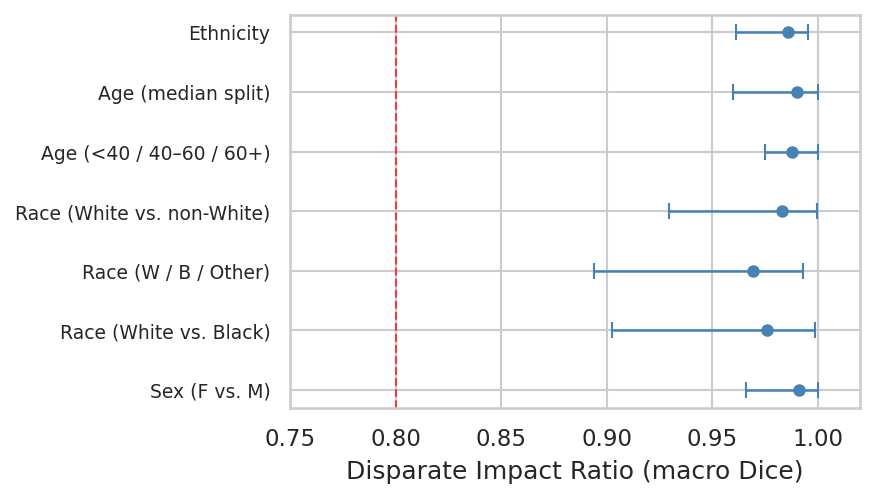
\includegraphics[width=0.525\textwidth]{dir_forest_global.png}\hfill
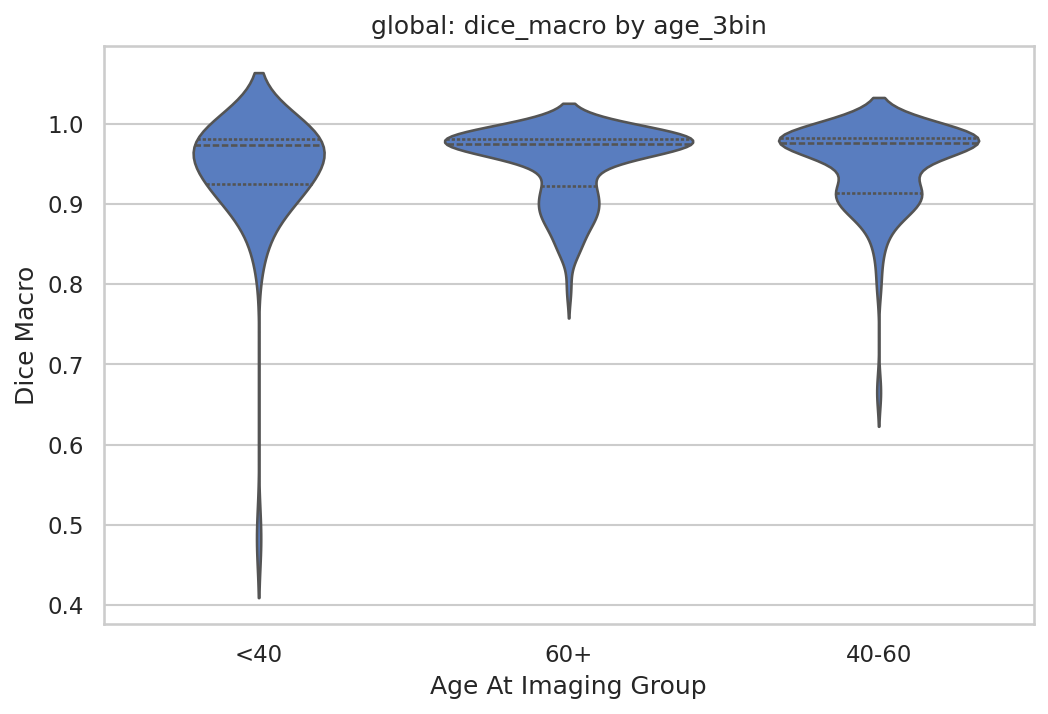
\includegraphics[width=0.455\textwidth]{violin_dice_macro_age.png}
\caption{Global fairness audit of $M_{\mathrm{mix}}$ on the full $228$-case test
set. \textbf{Left:} Forest plot of disparate impact ratios across all seven
demographic groupings and three metrics; point estimates (dots) with BCa $95\%$
bootstrap confidence intervals (whiskers). The dashed line marks the four-fifths
adverse-impact threshold ($0.80$); every lower bound clears it comfortably.
\textbf{Right:} Distribution of macro Dice by age bin ($n = 45$, $86$, $97$).
Medians are nearly identical (${\sim}0.974$); the youngest bin carries a wider
lower tail (a handful of difficult cases), but the overall age effect is negligible
($\varepsilon^2 < 0.01$, $p_{\mathrm{fdr}} = 0.98$).}
\label{fig:global_audit}
\end{figure}

\subsection{Biased Ruler Effect}
\label{sec:biased_ruler}

We now ask whether the choice of reference label can change a fairness verdict.
The global audit of ``\nameref{sec:global}'' found $M_{\mathrm{mix}}$ fair across
all three attributes ($0/63$ FDR-significant tests, all DIRs $> 0.96$) -- but that
verdict rests on expert labels. What happens if we replace the ruler?
We take the same model, the same $76$ gold-test images, and
score them twice: once against the expert (gold) labels -- the ground truth --
and once against $M_{\mathrm{gold}}$'s predictions on those same images, which
serve as the generated-silver ruler described in ``\nameref{sec:design}''.
Because the predictions are identical and only the reference label changes, any
difference in the fairness verdict is a pure ruler effect.

\paragraph{Performance gap between rulers.}
Against the gold ruler, $M_{\mathrm{mix}}$ achieves a macro Dice of $0.897$
(vertebral body $0.922$, disc $0.872$). Against the silver ruler the same
predictions score $0.973$ (vertebral body $0.979$, disc $0.968$) -- an inflation
of nearly $8$ percentage points. The gap itself is a first signal: the silver
ruler is far more lenient than the expert, because it shares systematic errors
with the model under test.

\paragraph{The verdict flip.}
Under the gold ruler, zero of the $63$ statistical tests reach significance after
Benjamini--Hochberg correction (smallest $p_{\mathrm{fdr}} = 0.13$) -- the model
is judged fair. Under the silver ruler, $11$ of $63$ tests are FDR-significant at
$\alpha = 0.05$, and every one of them is an age comparison (the three-bin and
median-split groupings, across Dice and nDSC for both structures and the macro
score). HD95 tells the same inflation story (gold mean $2.50$\,mm vs silver
$0.40$\,mm) but contributes no significant tests on either ruler, because its
heavy-tailed variance overwhelms the age signal on both.
The significance verdict reverses purely from the choice of reference
label. \autoref{tab:biased_ruler} summarises the two rulers side by side.

\begin{table}[t]
\centering
\caption{Biased-ruler comparison on the $76$ gold-test images (macro Dice).
The same predictions of $M_{\mathrm{mix}}$ are scored against two rulers: expert
labels (gold) and $M_{\mathrm{gold}}$'s predictions (silver). DIR and DPD are
rate-based (threshold $\tau = 0.8$); $p_{\mathrm{fdr}}$ is the Kruskal--Wallis
test after Benjamini--Hochberg correction. The silver ruler saturates
(DIR~$\equiv 1.0$, zero failures above $\tau$) while simultaneously producing
significance on the continuous test for age.}
\label{tab:biased_ruler}
\small
\begin{tabular*}{\textwidth}{@{\extracolsep{\fill}} l c c c c c c}
\hline\noalign{\smallskip}
 & \multicolumn{3}{c}{Gold ruler} & \multicolumn{3}{c}{Silver ruler} \\
\noalign{\smallskip}\cline{2-4}\cline{5-7}\noalign{\smallskip}
Grouping & DIR & DPD & $p_{\mathrm{fdr}}$ & DIR & DPD & $p_{\mathrm{fdr}}$ \\
\noalign{\smallskip}\hline\noalign{\smallskip}
Sex          & $1.000$ & $0.000$ & $0.997$ & $1.000$ & $0.000$ & $0.718$ \\
Race (W/B)   & $0.956$ & $0.044$ & $0.997$ & $1.000$ & $0.000$ & $0.328$ \\
Age (3 bins) & $0.952$ & $0.048$ & $0.270$ & $1.000$ & $0.000$ & $0.026^{\ast}$ \\
\noalign{\smallskip}\hline
\end{tabular*}

\smallskip
{\footnotesize $^{\ast}$\,Significant after FDR correction at $\alpha = 0.05$.
All $11$ significant tests on the silver ruler are age groupings (three-bin and
median split, Dice and nDSC).}
\end{table}

\paragraph{Mechanism: false confidence via variance collapse.}
The verdict flip does not arise because the silver ruler reveals a larger gap --
it does the opposite. The age trend is smaller against silver than against
gold: median macro Dice drops from $0.925$ ($<$40) to $0.898$ (60+) on the gold
ruler (a $2.7$-point spread) but only from $0.980$ to $0.974$ on silver (a
$0.6$-point spread). What changes is the within-group variance. Recall that the
silver ruler is $M_{\mathrm{gold}}$'s predictions -- so scoring against it
measures inter-model agreement rather than accuracy. That agreement sits at
${\sim}0.97$ Dice, far above the ${\sim}0.89$ that the same predictions achieve
against the expert labels, and the standard deviation across the $76$ cases drops
from $0.058$ (gold) to $0.014$ (silver) -- a ${\sim}4\times$ reduction. We attribute
this high agreement to the inherent simplicity of cervical-spine segmentation --
vertebral bodies and discs are large, high-contrast structures with well-defined
boundaries -- combined with the shared architecture and training recipe, which
lead both models to converge on similar solutions regardless of the specific
training cases.\footnote{$M_{\mathrm{mix}}$ and $M_{\mathrm{gold}}$ do share $288$
training cases, but this is not the primary driver: even
$M_{\mathrm{gold}}$ and $M_{\mathrm{silver}}$, trained on fully disjoint data
(zero case overlap), still agree at $0.97$ macro Dice on the same $76$ images.
The high inter-model agreement is a property of the task, not of shared
training data.} The Kruskal--Wallis test's power
scales with signal-to-noise, so the same clinically negligible age gradient that
is buried in gold's noise ($H = 7.0$, $p = 0.030$,
$p_{\mathrm{fdr}} = 0.27$) clears correction once silver's collapsed variance
sharpens the ranks ($H = 11.4$, $p = 0.003$, $p_{\mathrm{fdr}} = 0.026$). The
ruler did not change the patient; it changed the test's power.
A threshold sensitivity sweep confirms the saturation: the silver DIR remains
pinned at $1.0$ for all groupings through $\tau = 0.85$ and only drops (to
$0.97$) at $\tau = 0.90$, whereas the gold DIR already flags age disparity at
$\tau = 0.70$ and collapses to $0.57$ at $\tau = 0.90$.
\autoref{fig:biased_ruler} visualises the variance collapse: the same downward
staircase appears on both rulers, but gold's wide boxes bury the signal while
silver's razor-thin boxes expose it.

\paragraph{Comparison with Parikh et al.}
Parikh et al.~\cite{parikh2025labelbias} show a biased-ruler effect in
breast-MRI segmentation where the silver ruler makes a real gap look larger
than it truly is (DIR drops from $0.871$ to $0.815$). Our silver ruler does
something different: it leaves the gap the same size (or even shrinks it) but
makes a negligible gap look statistically significant. In their case, the ruler
exaggerates the signal; in ours, it removes the noise that would otherwise mask
it. Both lead to the same practical problem -- the fairness verdict depends on
which reference label you choose -- but through opposite routes.

\paragraph{The age effect is intrinsic.}
Although the significance is a ruler artifact, the underlying age trend is not.
It appears on both rulers in the same direction (60+ worst), is
consistent with the degenerative anatomy documented in
``\nameref{sec:confounders}'' (vertebral merging in older spines), and is
independently corroborated by the encoder probe
(``\nameref{sec:probing_results}''). An effect visible through the true ruler, the
correlated ruler, and the learned representation is unlikely to be a label
artifact -- it reflects intrinsic difficulty in older spines.

\paragraph{Not unfairness.}
A statistically significant gap is not the same as an unfair model. The
magnitudes here are clinically negligible: the worst-vs-best age group spans
$2.7$ Dice points on gold ($0.925 \to 0.898$) and $0.6$ points on silver, with
every patient receiving a ${\sim}0.90$+ Dice segmentation. All gold-ruler DIRs
exceed $0.94$ -- far above the four-fifths threshold -- and no subgroup is failed
by any practical measure. The contribution of this experiment is methodological:
it demonstrates that a machine-generated reference label can manufacture a
finding out of a non-issue, and that significance alone should not be read as
evidence of harm.

\begin{figure}[t]
\centering

\includegraphics[width=\textwidth]{age_trend_gold_vs_silver.png}
\caption{The variance-collapse mechanism behind the verdict flip. Both panels
show macro Dice by age bin for the same $76$ predictions of $M_{\mathrm{mix}}$,
scored against the gold ruler (left) and the silver ruler (right). The age
gradient runs in the same direction on both (60+ worst), but the gold ruler's
per-group standard deviations ($0.03$--$0.10$) bury the signal below FDR
correction, while the silver ruler's collapsed variance ($0.01$--$0.02$) exposes
it. The ruler changed the test's power, not the patient's outcome.}
\label{fig:biased_ruler}
\end{figure}

\subsection{Bias Amplification}
\label{sec:amplification}

The biased-ruler experiment showed that the choice of reference label can distort
a fairness verdict at evaluation time. We now ask whether label provenance in
training can do the same. E3 and E4 (\autoref{tab:experiments}) compare
the three models -- $M_{\mathrm{mix}}$, $M_{\mathrm{gold}}$, and
$M_{\mathrm{silver}}$ -- on the same $76$ gold-test cases scored against expert
labels, so any difference in fairness is attributable to the training labels
alone.

\paragraph{Segmentation quality.}
$M_{\mathrm{silver}}$ achieves a macro Dice of $0.897$ (vertebral body $0.921$,
disc $0.872$) -- identical to $M_{\mathrm{mix}}$ to three decimal places despite
never seeing an expert label during training. $M_{\mathrm{gold}}$ scores slightly
lower ($0.888$; vertebral body $0.914$, disc $0.862$), likely because it trains on
fewer cases ($288$ versus $450$ and $798$). Silver training labels do not degrade
absolute performance in this setting; the larger training pool compensates for the
noisier supervision.

\paragraph{Fairness verdict.}
\autoref{tab:amplification} reports the macro Dice DIR for all three models. Zero
of the $63$ statistical tests reach significance after Benjamini--Hochberg
correction on any model (smallest $p_{\mathrm{fdr}} = 0.061$,
$M_{\mathrm{gold}}$ nDSC disc by age). The
$M_{\mathrm{silver}}$ DIRs are nearly identical to $M_{\mathrm{mix}}$ -- in most
groupings the values coincide exactly -- and all exceed $0.93$. If anything,
$M_{\mathrm{gold}}$ is the least fair of the three on the disc (race W/B/O DIR
$= 0.813$ versus $0.875$ for both $M_{\mathrm{mix}}$ and $M_{\mathrm{silver}}$),
though even that value clears the four-fifths threshold. There is no evidence that
silver training labels amplify demographic bias.

\begin{table}[t]
\centering
\caption{Bias amplification: macro Dice DIR for the three models on the $76$
gold-test cases (expert reference). DIR $= 1.0$ denotes parity; the four-fifths
threshold is $0.80$. $M_{\mathrm{silver}}$ matches $M_{\mathrm{mix}}$ almost
exactly; $M_{\mathrm{gold}}$ is occasionally worse. All values exceed
$0.80$; $0/63$ tests reach FDR significance on any model.}
\label{tab:amplification}
\small
\begin{tabular*}{\textwidth}{@{\extracolsep{\fill}} l c c c}
\hline\noalign{\smallskip}
Grouping & $M_{\mathrm{mix}}$ & $M_{\mathrm{gold}}$ & $M_{\mathrm{silver}}$ \\
\noalign{\smallskip}\hline\noalign{\smallskip}
Sex          & $1.000$ & $0.946$ & $1.000$ \\
Race (W/B)   & $0.956$ & $0.994$ & $0.956$ \\
Race (W/B/O) & $0.938$ & $0.938$ & $0.938$ \\
Age (3 bins) & $0.952$ & $0.956$ & $0.952$ \\
Age (median) & $0.998$ & $0.996$ & $0.998$ \\
\noalign{\smallskip}\hline
\end{tabular*}
\end{table}

\paragraph{Interpretation.}
The null result is expected: bias amplification requires both an underlying
disparity for noisy labels to exaggerate and a silver source that is
differentially biased across groups. Neither precondition holds here. The global
audit (``\nameref{sec:global}'') already found no demographic gap to amplify
($0/63$, all DIRs $> 0.96$), and the silver labels are high-quality -- Zhou et
al.~\cite{zhou2025cspineseg} selected which exams to expert-annotate
pseudo-randomly (by medical record number), leaving the gold and silver pools
demographically comparable, so the machine-generated labels carry no systematic
group-level bias for training to propagate.
This contrasts with Parikh et al.~\cite{parikh2025labelbias}, who observed $66\%$
gap widening (DIR dropping below $0.80$) when training on their silver labels. The
difference lies in the preconditions: their silver annotator was an independently
trained model that was itself biased against younger patients, acting on a task
with a substantial pre-existing age disparity. In our setting, the silver labels
are produced by a model trained on a representative subset of the same
institution's gold annotations, segmenting large high-contrast structures whose
boundaries may leave little room for demographically differential error --
though we cannot test this hypothesis directly. The result suggests that
mixing silver labels into training is unlikely to harm fairness when the
underlying labels are well-calibrated and no pre-existing disparity exists for
noisy supervision to exaggerate.

\subsection{Demographic Probing}
\label{sec:probing_results}

The preceding experiments ask whether demographic groups receive different
outputs. We now ask a logically independent question: does the model's
internal representation carry demographic signal at all? Encoding a protected
attribute and producing a performance disparity are separate phenomena -- a model
can do one without the other~\cite{petersen2023feature}. The probe setup --
two encoders (nnU-Net bottleneck and MRI-CORE), each paired with a random-init
null, scored via PCA(50) and logistic regression in 5-fold CV -- is defined in
``\nameref{sec:probing_method}'' (\autoref{sec:probing_method}).

\paragraph{Results.}
\autoref{tab:probe} reports probe scores for all four encoder--null pairs across
three demographic attributes plus manufacturer (a sanity check). Sex is the most
strongly encoded attribute: the nnU-Net bottleneck reaches $0.957$ AUROC, with the
segmentation task contributing $+0.186$ above its random null ($0.771$). MRI-CORE
scores $0.931$, but its random-init null already achieves $0.836$ -- indicating
that ${\sim}90\%$ of the sex signal in the task-agnostic encoder comes from raw
pixel statistics (body silhouette, FOV extent) rather than learned anatomy. Age
is moderately encoded on both ($0.642$ nnU-Net, $0.632$ MRI-CORE), with task
training again the larger contributor ($+0.166$ vs.\ $+0.098$).
Race sits near chance on all encoders (wide CIs, fold variance $0.41$--$0.55$), consistent
with the null race finding in the fairness audit. Manufacturer reaches ${\sim}0.997$
universally -- a pixel-level scanner fingerprint independent of learned weights,
serving as a healthy end-to-end sanity check.

A confounder analysis on the full cohort confirms that the probe signals are not
artefacts of scanner assignment or attribute entanglement: sex $\times$
manufacturer ($\chi^2$ $p = 0.21$, Cram\'er's $V = 0.035$) and age $\times$ sex
($p = 0.08$, $r_{rb} = 0.07$) are not significant; age $\times$ manufacturer
reaches significance ($p = 0.02$) but at a negligible effect size
($r_{rb} = -0.09$), meaning older patients are only marginally more likely to
appear on one scanner -- too weak an association to account for the age probe
scores observed above.

\begin{table}[t]
\centering
\caption{Linear-probe scores for demographic attributes on frozen encoder
features ($n = 1{,}085$). ``Null'' denotes a random-initialised network of
identical architecture and preprocessing. $\Delta_{\mathrm{task}}$ is the
trained-minus-null gap, isolating the contribution of the training objective.
Sex is strongly encoded yet produces no performance disparity
(``\nameref{sec:global}''); age is the one axis with both encoding and a
(negligible) performance trend. Values are mean $\pm$ Nadeau--Bengio 95\% CI.}
\label{tab:probe}
\small
\begin{tabular*}{\textwidth}{@{\extracolsep{\fill}} l l c c c}
\hline\noalign{\smallskip}
Encoder & Attribute & Trained & Null & $\Delta_{\mathrm{task}}$ \\
\noalign{\smallskip}\hline\noalign{\smallskip}
nnU-Net        & Sex (AUROC)       & $0.957\pm.030$ & $0.771\pm.066$ & $+0.186$ \\
(segmentation) & Age (bal.\ acc.)  & $0.642\pm.023$ & $0.476\pm.055$ & $+0.166$ \\
               & Race (bal.\ acc.) & $0.491\pm.104$          & $0.373\pm.052$ & $+0.118$ \\
               & Manuf.\ (AUROC)   & $0.997\pm.004$          & $0.983\pm.012$ & $+0.014$ \\
\noalign{\smallskip}\cline{1-5}\noalign{\smallskip}
MRI-CORE       & Sex (AUROC)       & $0.931\pm.031$ & $0.836\pm.039$ & $+0.095$ \\
(task-agnostic) & Age (bal.\ acc.) & $0.632\pm.043$ & $0.534\pm.083$ & $+0.098$ \\
               & Race (bal.\ acc.) & $0.513\pm.071$ & $0.426\pm.064$ & $+0.087$ \\
               & Manuf.\ (AUROC)   & $0.997\pm.007$ & $0.992\pm.013$ & $+0.005$ \\
\noalign{\smallskip}\hline
\end{tabular*}
\end{table}

\paragraph{Encoding does not imply disparity.}
The central finding is a dissociation: sex is by far the most strongly encoded
attribute ($0.957$), yet the global audit found zero sex disparity ($0/63$
significant tests, DIR~$= 0.991$). The segmentation task has learned to exploit
sex-linked vertebral morphology -- larger bodies and discs in men, different canal
geometry -- without producing differential outcomes. Conversely, age is only
moderately encoded ($0.642$) yet is the one axis that shows a (clinically
negligible) performance trend, corroborating the biased-ruler finding that the age
effect is intrinsic anatomical difficulty rather than a label artefact. The probe
thus confirms that encoding is neither necessary nor sufficient for disparity: a
model can strongly represent a demographic feature and still be fair, because the
decoder maps those different representations to equally accurate outputs.
\section{Discussion}

% TODO:
% - [ ] Model Bias vs anatomical difference: key findings discussed here
% - [ ] Danger of automated labels
% - [ ] Key takeaways, recommendations

\section{Conclusion}

Cervical-spine MRI segmentation lacked a fairness audit across multiple
demographic axes. We conducted one on the CSpineSeg dataset ($1{,}254$ exams),
evaluating performance across sex, race, and age with anatomically informed
metrics.

The model is fair by every measure we applied: $0/63$ statistical tests reach
significance after FDR correction, all disparate impact ratios exceed $0.96$, and
demographics collectively explain $1.3\%$ of Dice variance. Replacing expert
reference labels with machine-generated ones flips the verdict for age --
not by inflating the gap but by collapsing within-group variance ${\sim}4\times$,
a false-confidence mode complementary to the false-magnitude effect of Parikh et
al.~\cite{parikh2025labelbias}. Training on silver labels does not amplify
demographic bias in this anatomy, unlike the amplification observed in breast
MRI~\cite{parikh2025labelbias}. Encoder probing confirms that the residual age
gradient reflects intrinsic anatomical difficulty -- older spines are harder to
segment -- rather than algorithmic harm, and that strong encoding of a protected
attribute (sex, AUROC $0.957$) need not produce any performance disparity.

These results carry two practical implications. First, reference-label provenance
is a first-order confounder in fairness evaluation: the same predictions, scored
against different labels, yield opposite conclusions. Any fairness claim must
state where its ruler comes from. Second, debiasing a model's learned
representations without first confirming an output-level disparity addresses a
problem that may not exist -- our model strongly encodes sex yet exhibits no
sex-based performance gap.

Our audit is limited to a single institution, anatomy, and architecture, and the
high-performance ceiling of cervical vertebral bodies and discs leaves little room
for disparity to emerge. Whether these findings generalise to harder anatomies or
lower-performing models remains open. We hope this work opens a rigorous
conversation about fairness in spine MRI segmentation.


% ---- Bibliography ----
%
% BibTeX users should specify bibliography style 'splncs04'.
% References will then be sorted and formatted in the correct style.
%
\bibliographystyle{splncs04}
\bibliography{mybibliography}
%
% Do check for citation formatting using Google Scholar
%
\end{document}
